\chapter{DEPLOYMENT AND MAINTAINENCE}

\section{Installation and Uninstallaion}
\subsection{Installing}
\begin{itemize}
\item Get the latest copy of KWEST by downloading from the project hosting site: \url{https://code.google.com/p/kwest/downloads}
\item After extracting the contents, open up a terminal and type in the following commands:
\begin{lstlisting}[language=bash,frame=single]
make kwest_libs
export LD_LIBRARY_PATH=../lib:D_LIBRARY_PATH
make
\end{lstlisting}
\end{itemize}

\subsection{Mounting and Unmounting}
\begin{itemize}
\item To mount a KWEST file system, the user needs to run the \textit{mount} script which will mount the file system in the specified folder. 
\begin{lstlisting}[language=bash,frame=single]
./kwest mount-point
\end{lstlisting}
\item To unmount a KWEST file system, the user needs to run the \textit{fusermount -u} command with the argument \textit{path of KWEST mount point}. A successful unmount operation does not return any message.
\begin{lstlisting}[language=bash,frame=single]
fusermount -u mount-point
\end{lstlisting}
\end{itemize}

\subsection{Uninstallation and Removal of Data}
\begin{enumerate}
\item KWEST ``installs'' files in the users local directory.
\item To clean all the installation data including the database and log files, the user should use the \emph{make clean} or \emph{make ob} commands.
\item These commands are present in the Makefile, which comes with the project source.
\item In case of manual installation, there is a \emph{KWEST} folder in the \emph{.config} directory.
\item Incomplete removal of files may cause haphazard execution of the program or corruption of files.
\end{enumerate}

\newpage
\section{User Help}

KWEST is a virtual file system. This means that the folders and files represented by it are a part of its virtual organisation. Each file in KWEST represents an actual file stored somewhere on the underlying file system. The main focus of using KWEST is organisation.

\subsection{Importing Files and Folders}

\begin{itemize}
\item By default KWEST imports from the users \textbf{HOME} folder. It recursively scans all the sub folders and imports the folder hierarchy into KWEST. Hidden files are ignored by KWEST.

\item The user can also explicitly use the \textbf{import} tool to import files and folders into KWEST. The import tool accepts the folder to import as argument and imports all files and folders within it. It can work regardless of whether the KWEST file system is mounted or not.

\item While importing, the metadata of the file is used to organise each file. For e.g.: A music file contains the song's artist, which is used to categorise that file.
\end{itemize}

\section{Browsing Files by Type}

\subsection{Audio}
This folder contains all the files recognised by the system as being of type audio. Upon accessing the folder, each Audio file is further categorised by \textbf{Album}, \textbf{Artist}, \textbf{Genre}. If a particular metadata is absent for the audio file, KWEST categorises it in the Unknown folder. \newline
For e.g. If the audio file does not have any artist associated with it, it can be found in \textbf{UnknownArtist}.
\begin{figure}[htb]
\centering
\setlength\fboxsep{0pt}
\setlength\fboxrule{0.5pt}
\fbox{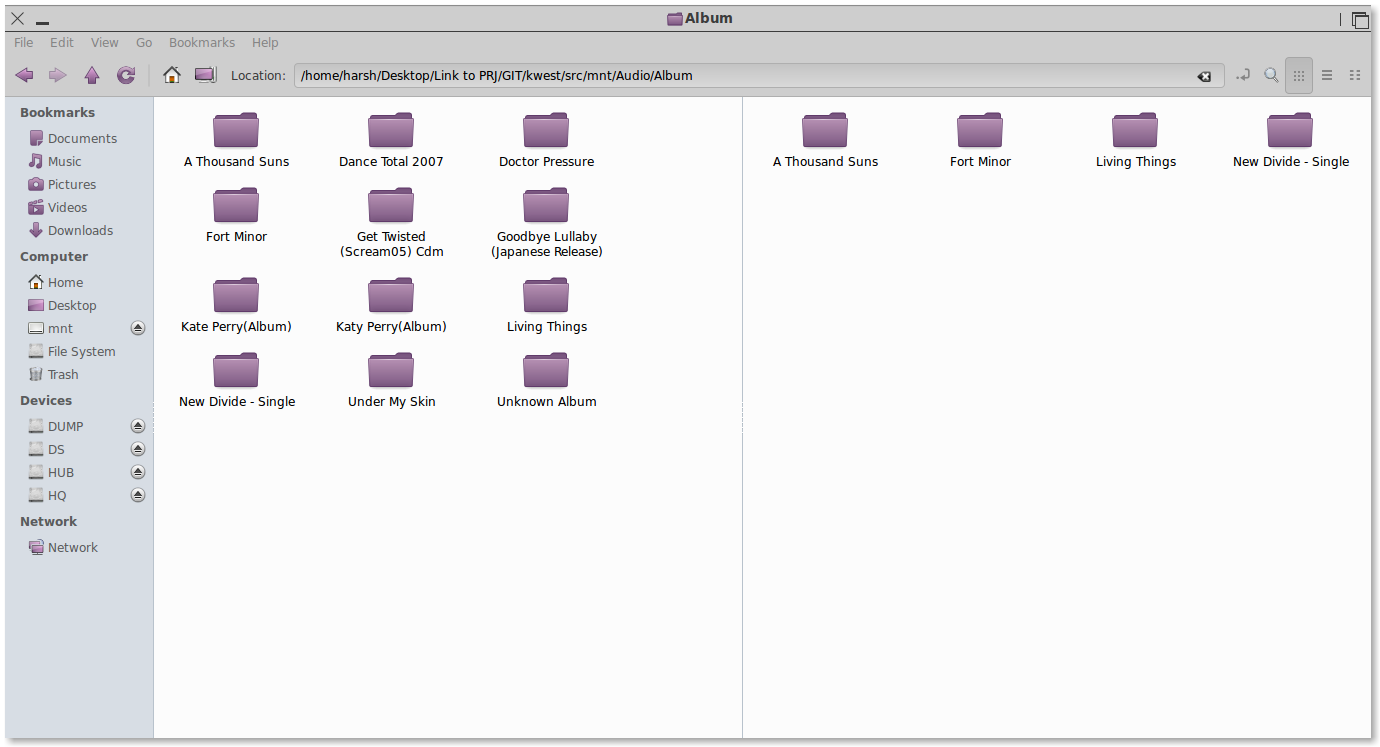
\includegraphics[width=0.8\linewidth]{./opimg/nemo_audiodual.png}}
%\includegraphics[width=0.8\textwidth]{image.png}
\caption{Audio files being categorised by /Album and /Artist/Album views}
\label{fig:dfd0}
\end{figure}

\subsection{Image}
This folder contains all the image files recognised by the system. Inside, the images are organised by ImageCreator and ImageDate. 
The ImageCreator sub folder is based on \textit{Creators} like software - Adobe Photoshop, or hardware - Camera Models. Each ImageCreator tag is further organised by ImageDate. 
The ImageDate folder contains images sorted by \textit{Month-Year} of creation. E.g.: A picture taken on ``\textit{2nd March 1992}'' will appear under ``\textit{1992Mar}''.
As with Audio, files with metadata missing will appear under appropriate \textit{Unknown} sub folders.
\begin{figure}[htb]
\centering
\setlength\fboxsep{0pt}
\setlength\fboxrule{0.5pt}
\fbox{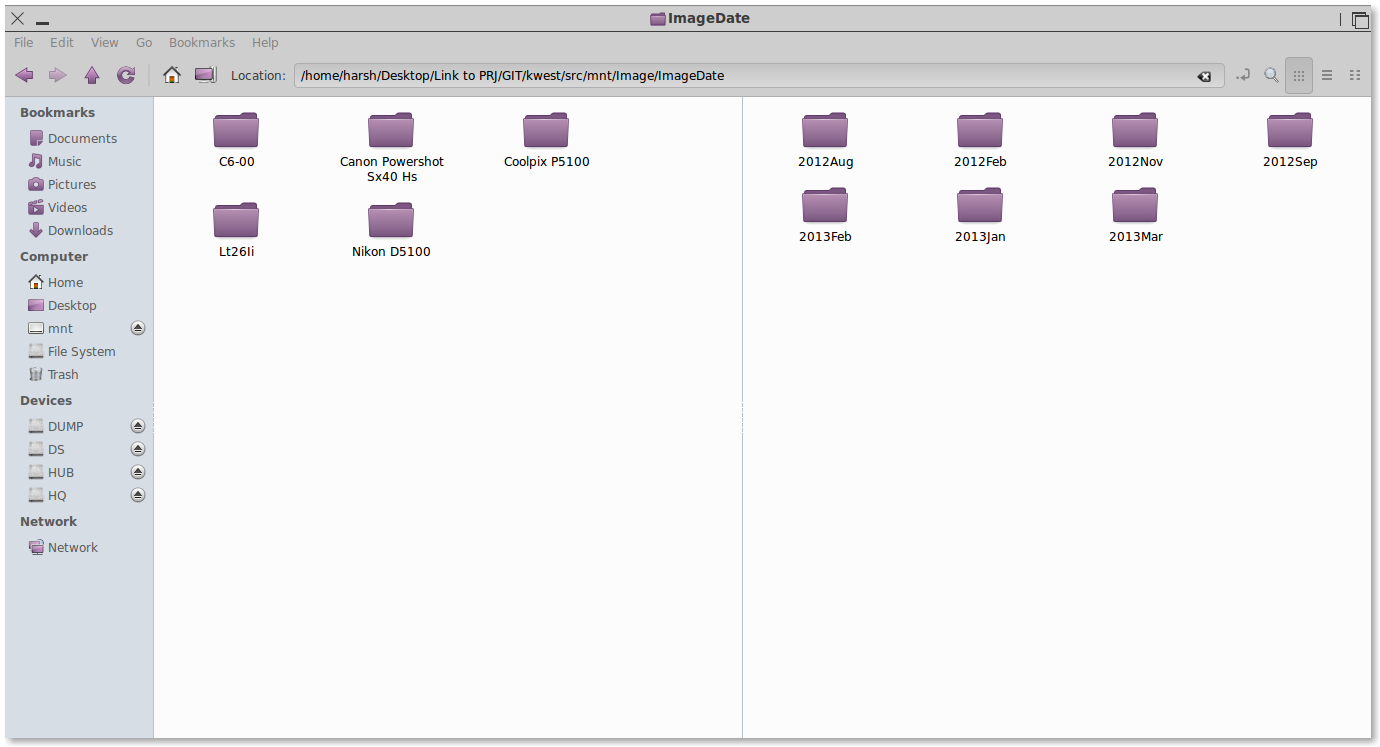
\includegraphics[width=0.8\linewidth]{./opimg/nemo_imagesort.png}}
%\includegraphics[width=0.8\textwidth]{image.png}
\caption{Images being categorised by Creator and CreationDate}
\label{fig:dfd0}
\end{figure}

\subsection{PDF}
All PDF documents are tagged with the PDF tag. Each PDF document is organised by its \textit{Author,Publisher,Subject} and \textit{Title}. Files with metadata missing are appropriately tagged under \textit{Unknown} tags.
\begin{figure}[htb]
\centering
\setlength\fboxsep{0pt}
\setlength\fboxrule{0.5pt}
\fbox{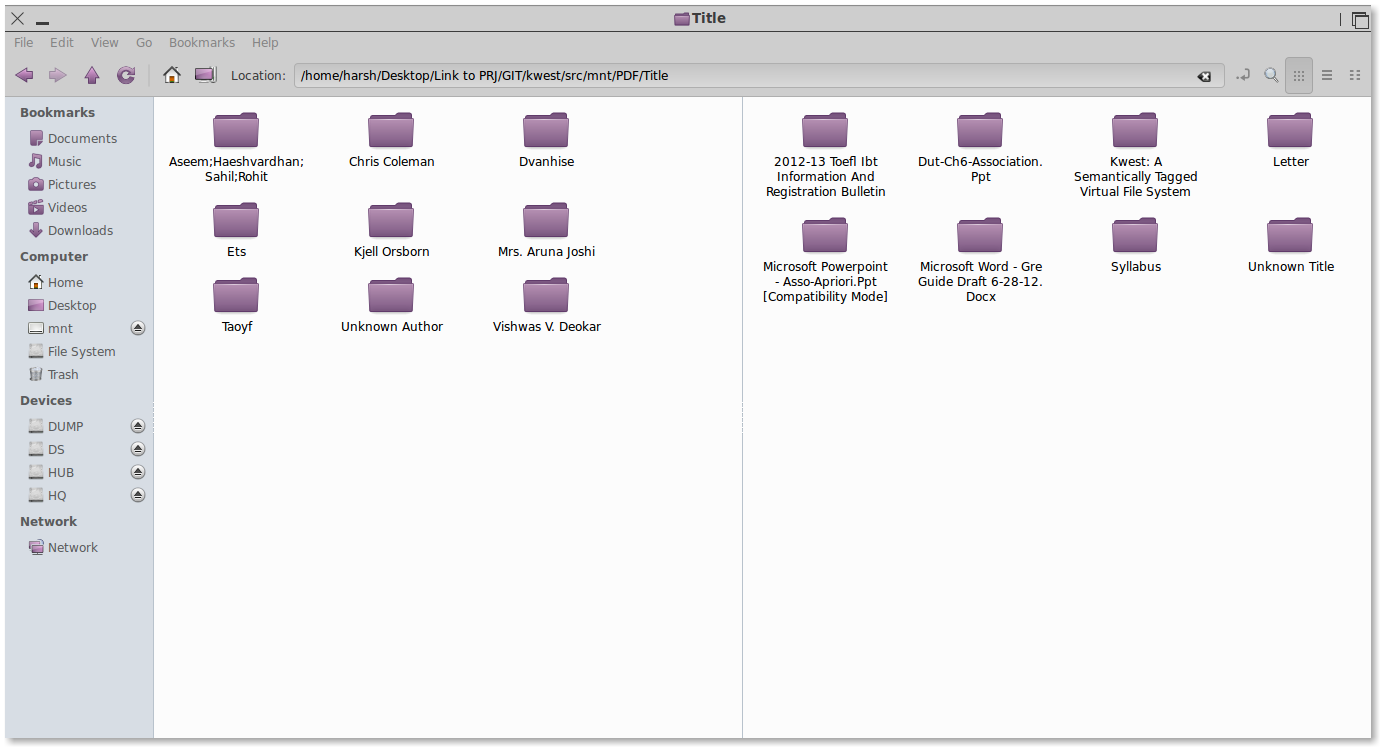
\includegraphics[width=0.8\linewidth]{./opimg/pdfsort.png}}
%\includegraphics[width=0.8\textwidth]{image.png}
\caption{PDF documents being separated by Author and Title}
\label{fig:dfd0}
\end{figure}

\subsection{Video}
Currently, the system organises video based only on Length, with the categories being \textit{Short, Medium and Long}. A short video is anything with less than 1800s of playtime. Videos with play time equal to or greater than 5400s are considered Long, and anything between them is considered Medium. The Video tag does not contain any categories as most of the videos stored by the user do not have any metadata present.
\begin{figure}[htb]
\centering
\setlength\fboxsep{0pt}
\setlength\fboxrule{0.5pt}
\fbox{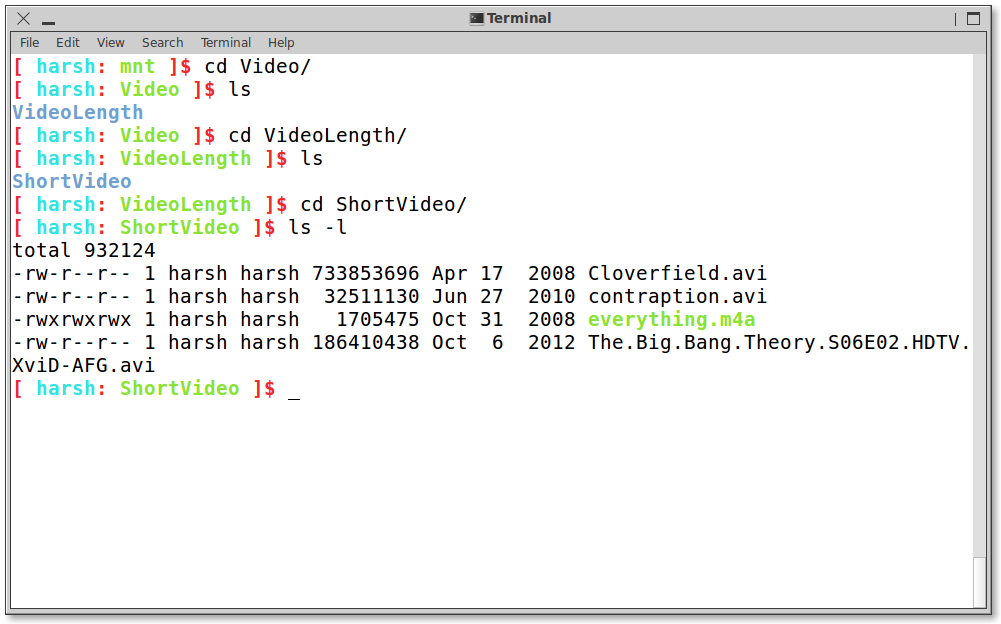
\includegraphics[width=0.8\linewidth]{./opimg/term_video.png}}
%\includegraphics[width=0.8\textwidth]{image.png}
\caption{Browsing the KWEST Video folder in a terminal}
\label{fig:dfd0}
\end{figure}

\subsection{USER}
The tag \textbf{`USER'} refers to the \textit{username} of the current user. The user can create and manage his own personal tags in this folder.
\begin{figure}[htb]
\centering
\setlength\fboxsep{0pt}
\setlength\fboxrule{0.5pt}
\fbox{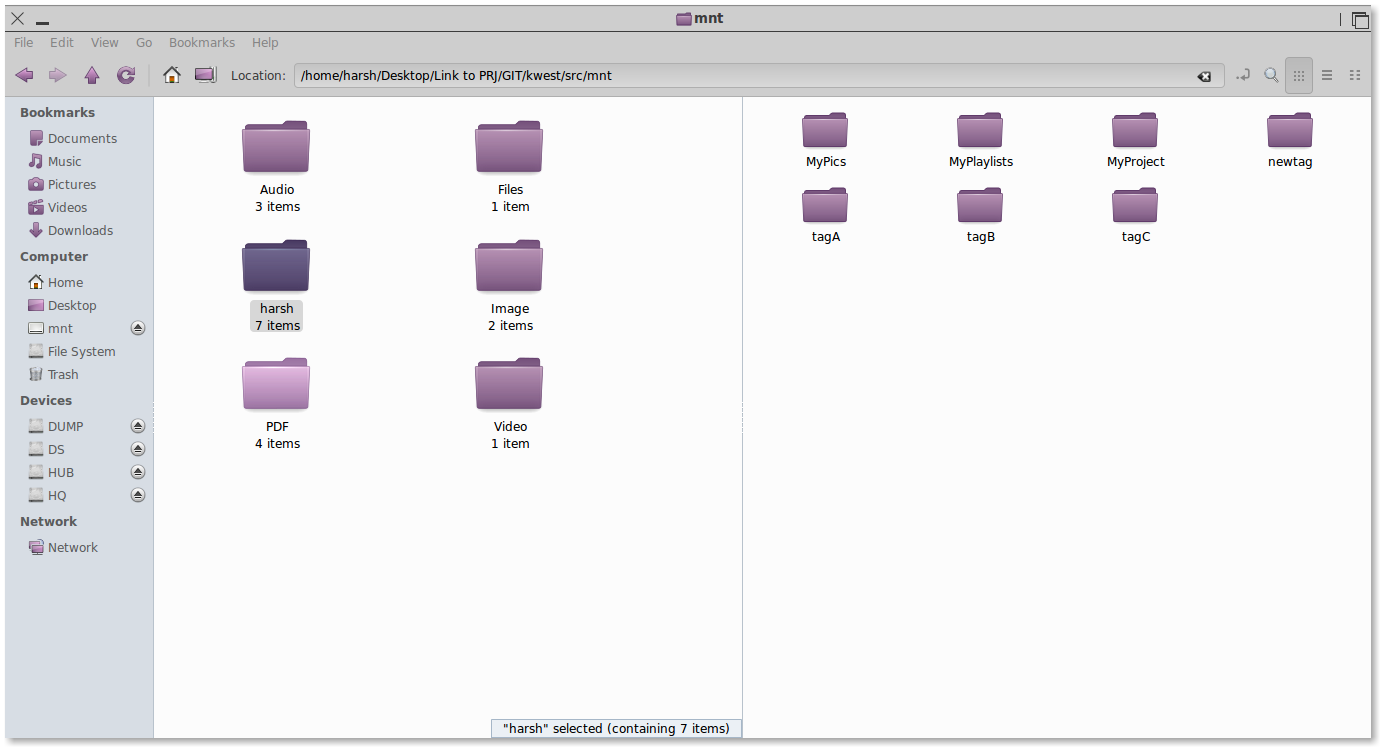
\includegraphics[width=0.8\linewidth]{./opimg/usertags.png}}
%\includegraphics[width=0.8\textwidth]{image.png}
\caption{User tags displayed in KWEST}
\label{fig:dfd0}
\end{figure}


\subsection{Using Suggestions to tag files}
KWEST helps the user with organisation by providing suggestions for tagging files. These suggestions are provided as files prefixed with the word - ``\textit{SUGGESTED}''. The user may make use of that suggestion by tagging that file in the current tag. \newline
e.g. in tag \textit{Zodiac}, there are 3 suggestions: \textit{ARIES, GEMINI, CANCER} each shown as a file with \textit{SUGGESTED} prefixed in their names. To make use of the suggestion on \textit{ARIES}, the user tags the file \textit{ARIES} under the tag \textit{Zodiac}. The file is now seen in the tag without the suggested prefix. The other suggestions are still present and may be used further or deleted.
\begin{figure}[htb]
\centering
\setlength\fboxsep{0pt}
\setlength\fboxrule{0.5pt}
\fbox{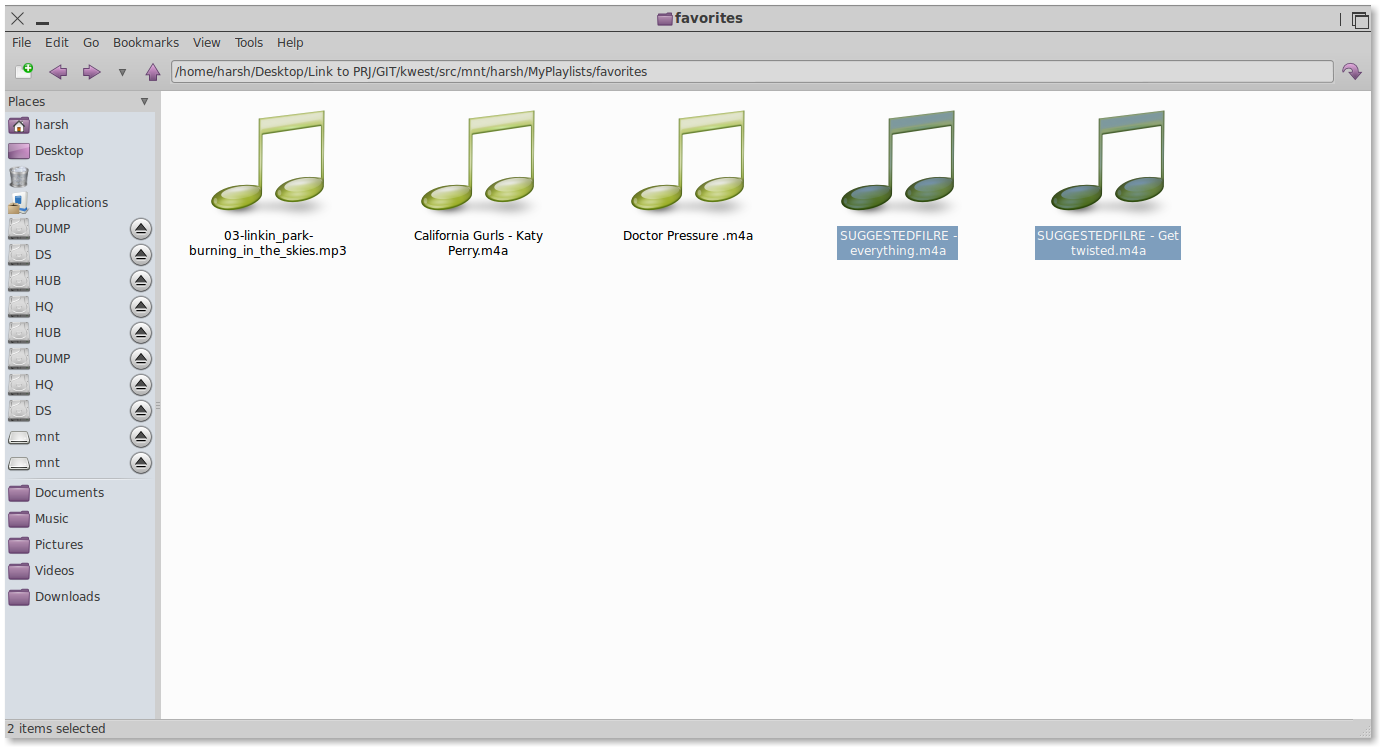
\includegraphics[width=0.8\linewidth]{./opimg/suggestions.png}}
%\includegraphics[width=0.8\textwidth]{image.png}
\caption{KWEST offering suggestions for tag favourites}
\label{fig:dfd0}
\end{figure}
